
\clearpage
\section{La fonction d'acquisition}

La fonction d'acquisition soutient l'utilisateur lors de la gestion de procédures d'acquisition petites et grandes. Le module d'acquisition comprend :

\begin{itemize}
\item la création de l'acquisition,
\item l'examen de l'offre,
\item la procédure d'adjudication,
\item l'approbation de l'adjudication et
\item les contrats.
\end{itemize}

\vspace{\baselineskip}

De plus, il est possible de travailler en suivant différents modèles :

\begin{itemize}
\item Acquisitions de gré à gré (avec un ou plusieurs soumissionnaires).
\item Acquisitions sur invitation ou procédures ouvertes.
\end{itemize}

\vspace{\baselineskip}

Vu que les déroulements d'acquisitions diffèrent d'une entreprise à l'autre ou d'un projet à l'autre au sein d'une même entreprise, ce module (Procédure d'acquisition) est fait sur mesure et documenté selon les processus de chaque client. Dans ce chapitre, des déroulements possibles de procédures d'acquisitions sont suivis et documentés à titre d'exemple.

\vspace{\baselineskip}

\textbf{Introduction :}

Afin de faciliter l'organisation, les acquisitions (invitations / appels d'offres), offres, et contrats sont numérotés. Lors de la création de ces éléments, vous serez menés à établir leurs liens (quelle offre concerne quelle acquisition, quel contrat concerne quelle offre). La numérotation est ensuite composée en fonction :

\vspace{\baselineskip}

L'acquisition n. 28 avec l'offre correspondante n. 45 donne dans la liste des offres le numéro 28.45. Si le contrat n. 31 vient s'y ajouter, ceci donne le numéro 28.45.31 dans la liste des contrats. Les numéros sont fixés automatiquement par CUBE PA.

\subsection{Flux de travail pour acquisitions de gré à gré}

Ce flux de travail peut être employé pour des procédures avec un ou plusieurs soumissionnaires. \\
Le flux de travail comporte les étapes suivantes :

\begin{enumerate}
\item Préparation des documents pour l'appel d'offres
\item Initialisation de l'acquisition
\item Chargement des documents pour l'appel d'offres
\item Envoi de l'appel d'offres
\item Réception et chargement des offres
\item Établissement des PVs d'examen des offres et transmission à l'instance de décision
\item Approbation de la procédure par une position d'ordre supérieur
\item Établissement d'un contrat.
\end{enumerate}

Des états sont utilisés pour le suivi du progrès lors des procédures d'acquisition. Les états dans le tableau suivant décrivent un processus de projet typique.

\vspace{\baselineskip}

\begin{tabular}{|p{5cm}|p{9.5cm}|}    % p{9.5cm} l} %{cl}  % {|m{5.316cm}|m{9.586cm}|}
\hline
\textbf{État} & \textbf{Qui fixe l'état et sous quelles conditions} \\
\hline
Établissement de l'appel d'offres & Cet état est fixé automatiquement lorsqu'une acquisition est initialisée. \\
\hline
Approbation par X & Vous fixez cet état dès que X aurait vérifié l'appel d'offres. \\
\hline
Appel d'offres envoyé aux invités & Vous fixez cet état dès que vous aurez envoyé l'appel d'offres aux soumissionnaires (pour procédures de gré à gré 
et procédures sur invitation). \\
\hline
Examen des offres & Vous fixez cet état dès que vous aurez ajouté une offre. \\
\hline
Offre chez X & Vous fixez cet état une fois que vous aurez envoyé une offre avec son PV d'examen à X. \\
\hline
Décision position d'ordre supérieur & Vous fixez cet état une fois que vous aurez envoyé une offre avec son PV d'examen à X et qu'il est indiqué dans le PV d'examen qu'une décision doit être prise par une autorité politique. \\
\hline
Offre adjugée & X fixe cet état lorsque le chef de projet responsable ou l'autorité d'ordre supérieur aura approuvé l'adjudication \\
\hline
Contrat établi & X fixe cet état lorsque le contrat non signé aura été envoyé à l'adjudicataire \\
\hline
Signature X / Envoi & X fixe cet état lorsque le contrat signé par l'adjudicataire est envoyé au maître de l'ouvrage et au directeur général \\
\hline
Acquisition terminée & Vous fixez cet état une fois que vous aurez ajouté le contrat. \\
\hline
\end{tabular}

\vspace{\baselineskip}

Les états dans le tableau suivant décrivent une interruption ou un arrêt dans le progrès du projet :

\vspace{\baselineskip}

\begin{tabular}{|p{5cm}|p{9.5cm}|}    % p{9.5cm} l} %{cl}  % {|m{5.316cm}|m{9.586cm}|}
\hline
\textbf{État} & \textbf{Qui fixe l'état et sous quelles conditions} \\
\hline
Offre(s) refusée(s) / refusée(s) & Vous fixez cet état quand la direction du projet décide que cette offre ne sera plus suivie. La direction du projet peut aussi fixer cet état. \\
\hline
Offre renvoyée pour révision & Vous fixez cet état lorsque la direction du projet décide que cette offre doit être renvoyée pour révision. La direction du projet peut aussi fixer cet état. \\
\hline
\end{tabular}

\subsubsection{Étape 1: Préparation des documents pour l'appel d'offres}

Vous pouvez préparer les documents d'appel d'offres en utilisant Excel et Word, ou tout autre programme convenable.

\subsubsection{Étape 2: Initialisation de l'acquisition}

\begin{wrapfigure}[3]{l}{6.5cm}   % [x] Wie manche Zeile soll sich um die Grafik "brechen"
  \vspace{-35pt}      % Grundwert war 20; mit 30 schön oben beim Text ausgerichtet
  \begin{center}
    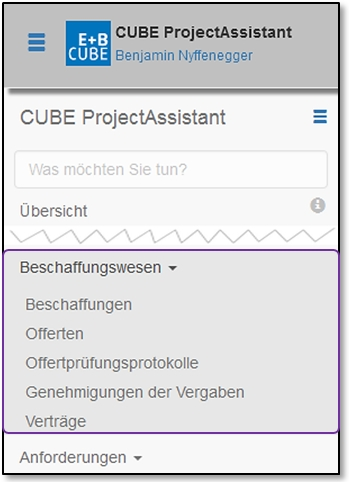
\includegraphics[width=1\linewidth]{../chapters/07_Beschaffungswesen/pictures/7-1-2_Menu_Beschaffungswesen.jpg}
  \end{center}
  \vspace{-20pt}
  \caption{Utiliser la fonction d'acquisition}
  \vspace{-10pt}
\end{wrapfigure}

Dans le menu à gauche, sélectionnez l'élément 'Fonction d'acquisition' et le sous-élément 'Acquisitions'. 

\vspace{5cm}

La liste des acquisitions s'affiche.

\vspace{2cm}

\begin{figure}[H]
\center{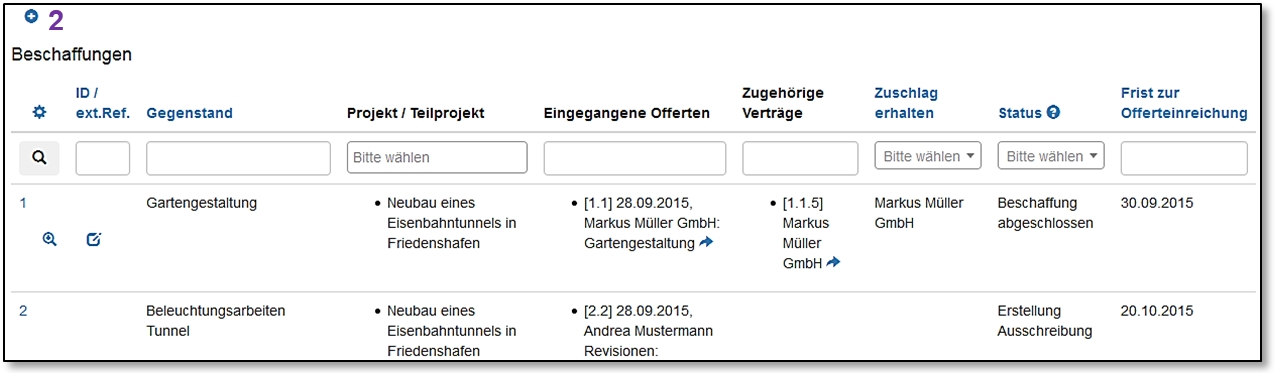
\includegraphics[width=1\linewidth]{../chapters/07_Beschaffungswesen/pictures/7-1-2_Beschaffung_Uebersicht.jpg}}
\caption{Aperçu des acquisitions}
% \label{fig:speciation}
\end{figure}

% Problem

% \pagebreak
Cliquez sur le symbole plus 
\includegraphics[height=12pt]{/Icons/Plussymbol.jpg} \col{(2)} en haut à gauche. Le masque de saisie d'une nouvelle acquisition s'affiche :

\vspace{\baselineskip}

Les champs obligatoires sont marqués par un astérisque *.

\begin{figure}[H]
\center{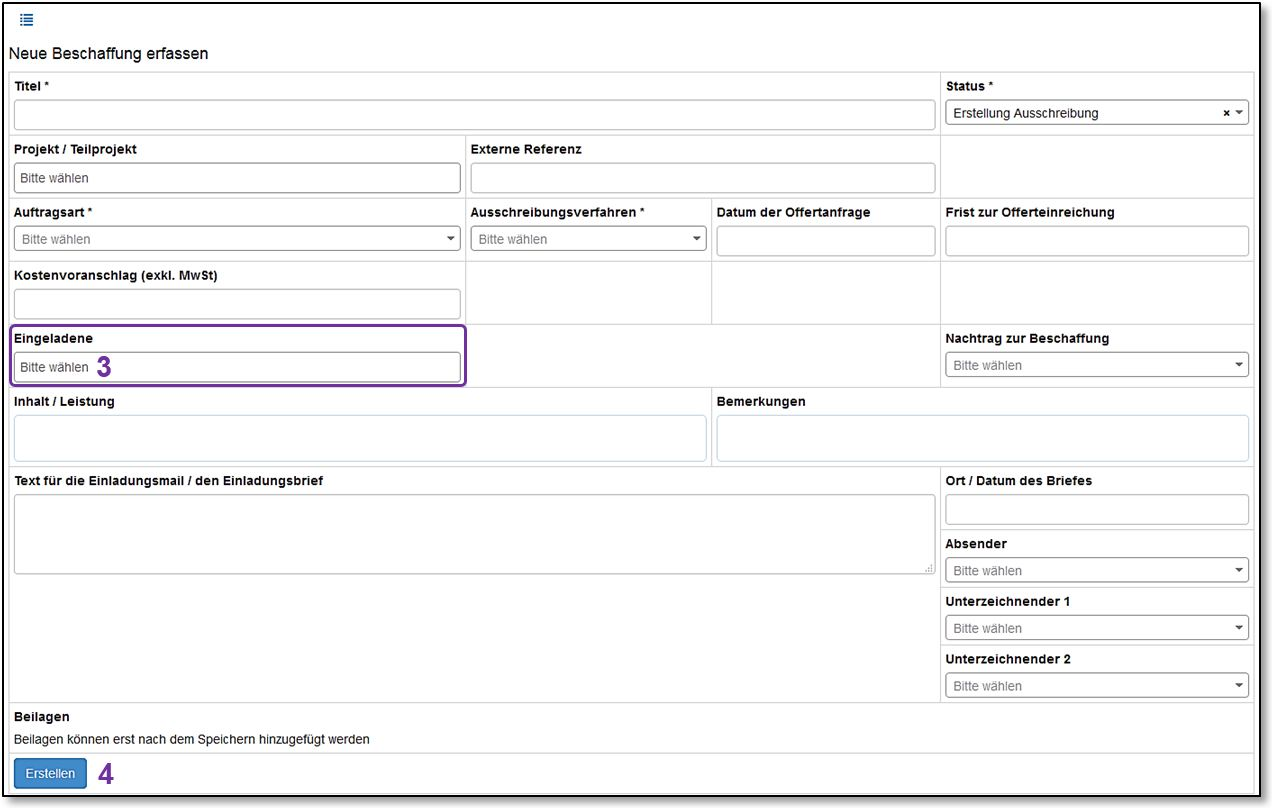
\includegraphics[width=1\linewidth]{712_BeschaffungErfassen.jpg}}
\caption{Saisir une nouvelle acquisition}
% \label{fig:speciation}
\end{figure}

Tout d'abord, vérifiez que le menu déroulant du champ 'Soumissionnaires invités' \col{(3)} comprend l'entreprise à laquelle vous souhaitez envoyer l'appel d'offres. Si ce n'est pas le cas, passez au module 'Configuration' dans le menu à gauche (voir chapitre \ref{bkm:Ref434830029}) et ajoutez-y l'entreprise (Des droits d'administrateur sont nécessaires pour cette étape. Contactez votre personne de contact CUBE PA). Si l'entreprise se trouve sur la liste, choisissez-la. Vous pouvez ensuite remplir le reste des champs :

\vspace{\baselineskip}

\begin{compactitem}
\item
Titre : Texte libre, court et concis.
\item
Etat : Automatiquement fixé à 'Établissement de l'appel d'offres' et doit rester ainsi.
\item
Projet / Sous-projet : Sélectionnez un ou plusieurs projet(s) ou sous-projet(s) correspondants.
\item
Référence externe : Ce champ est uniquement nécessaire pour la saisie rétroactive d'acquisitions qui se trouvaient sur une autre liste > à ne pas utiliser.
\item
Type de commande : Choisissez entre contrat de construction ou de services.
\item
Procédure d'appel d'offres : Sélectionnez 'de gré à gré'.
\item
Date de publication : Sélectionnez la date d'envoi de l'appel d'offres dans le calendrier.
\item
Délai de soumission : Sélectionnez le délai de soumission dans le calendrier.
\item
Devis : Si le devis est connu, vous pouvez saisir la somme. Vous pouvez uniquement utiliser des chiffres et un seul point. Vous aurez ensuite une comparaison directe entre le devis et l'offre.
\item
Supplément pour acquisition : Si l'acquisition que vous êtes en train d'établir consiste en un supplément pour une autre acquisition (ceci peut être la raison pour laquelle seul un soumissionnaire est invité), vous pouvez choisir l'acquisition de base de la liste.
\item
Contenu / Prestation : Courte description en texte libre des prestations attendues de l'adjudicataire, pas plus que 2 à 3 lignes.
\item
Remarques : Ici vous pouvez saisir en texte libre des conditions particulières pour cette acquisition (peut se faire aux prochaines étapes aussi).
\item
Texte pour e-mail / lettre d'invitation : Saisissez ici le texte de l'e-mail ou de la lettre d'invitation entier, à l'exception du lieu, de la date et de l'adresse. Vous pourrez ensuite générer un e-mail ou une lettre d'invitation complets à partir de ce contenu.
\item
Si vous souhaitez envoyer la lettre d'invitation sous forme papier, remplissez aussi les champs 'Date, lieu de délivrance' (texte libre), 'Expéditeur' (sélection de liste de l'entreprise qui expédie la lettre), 'Signature 1' (sélection de liste) et 'Signature 2' (sélection de liste). La 'signature 1' est hiérarchiquement plus importante, dans les cas où deux signatures sont requises.
\end{compactitem}

\vspace{\baselineskip}

Cliquez ensuite sur 'Créer' \col{(4)}, et vous aurez la possibilité d'ajouter des
pièces jointes :

\begin{figure}[H]
\center{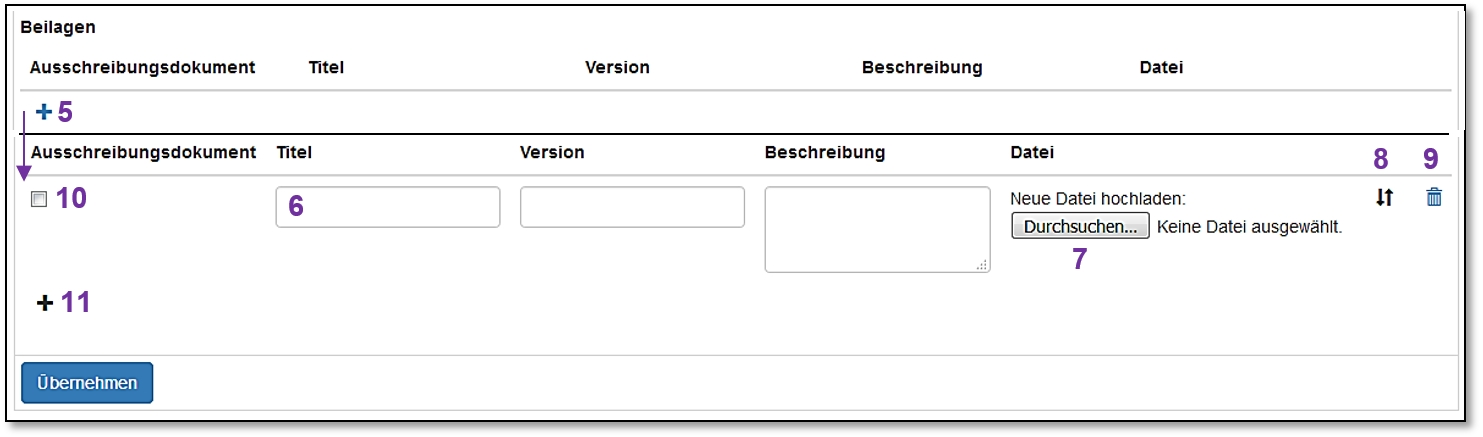
\includegraphics[width=1\linewidth]{../chapters/07_Beschaffungswesen/pictures/7-1-2_Beschaffung_Beilagen_hochladen.jpg}}
\caption{Ajouter des pièces jointes à une acquisition}
% \label{fig:speciation}
\end{figure}

Pour ajouter une pièce jointe, cliquez sur le symbole plus 
\includegraphics[height=12pt]{/Icons/Pluszeichen.jpg} \col{(5)}. Vous pouvez remplir les champs \col{(6)} et charger un fichier en cliquant 'Parcourir' \col{(7)}. Si vous avez chargé plusieurs pièces jointes, les flèches 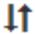
\includegraphics[height=12pt]{/Icons/VertPfeile.jpg} \col{(8)} vous permettent de modifier leur ordre (par glisser-déposer). Le symbole de poubelle 
\includegraphics[height=12pt]{/Icons/Muelltonne.jpg} \col{(9)} vous permet de supprimer une pièce jointe.
Si les documents chargés doivent pouvoir être téléchargés (lors de l'envoi de l'appel d'offre), cochez la case 'Document d'appel d'offre' \col{(10)}. Vous pouvez ajouter des documents additionnels par le moyen du symbole plus \includegraphics[height=12pt]{/Icons/pluszeichen.jpg} \col{(5)}. Terminez la procédure en cliquant 'Actualiser'.

\vspace{\baselineskip}

Vous pouvez ensuite soit passer directement à l'étape 3 soit y retourner plus tard.

\vspace{\baselineskip}

\textbf{Etape intermédiaire : Modifier une acquisition rétroactivement ou continuer avec une acquisition
après une interruption}

\vspace{\baselineskip}

Il n'est pas nécessaire de passer dans l'ordre des étapes 2 à 4. Il est également possible de modifier les données rétroactivement après avoir complété une étape. Vous pouvez toujours accéder à ces étapes depuis la liste des acquisitions. Choisissez l'élément de menu 'Fonction d'acquisition' puis le sous-élément 'Acquisitions'. La liste d'acquisitions s'affiche.

\vspace{\baselineskip}

Vous pouvez visuellement parcourir la liste ou la filter pour chercher l'acquisition souhaitée. Pour feuilleter la liste, utilisez les boutons au bas de la liste pour passer à la page précédente ou suivante ou à un numéro de page spécifique.

\begin{center}

\includegraphics[height=12pt]{/Icons/SeitenBlaettern.jpg}
\end{center}

Pour filtrer la liste, utilisez les champs de recherche sous l'en-tête des colonnes. Dans le champ 'ID / Ref. ext.', vous pouvais saisir un chiffre. L'identifiant est celui attribué par CUBE PA. Dans le champ 'Objet', vous pouvez saisir du texte libre. Le champ 'Projet/Sous-projet' contient une liste de sélection. Le champ 'Délai de soumission' dispose d'un calendrier. Une fois les chmaps de recherche remplis, cliquez sur le symbole de loupe 
\includegraphics[height=12pt]{/Icons/Lupe_kl.jpg} \col{(1)} à droite, et la liste filtrée s'affiche.

\begin{figure}[H]
\center{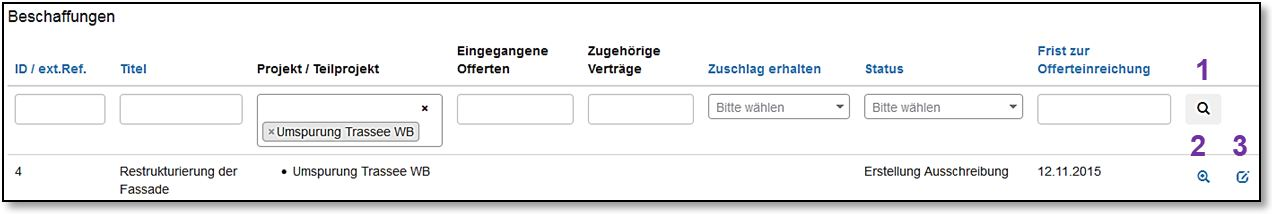
\includegraphics[width=1\linewidth]{712_BeschaffungFiltern.jpg}}
\caption{Utiliser le filtre pour chercher une acquisition}
% \label{fig:speciation}
\end{figure}

Si vous souhaitez uniquement visualiser l'acquisition, sans la modifier, cliquez sur le symbole de loupe bleu 
\includegraphics[height=12pt]{/Icons/Lupe.jpg} \col{(2)}. La saisie de l'acquisition est ouverte. Si vous cliquez sur le symbole de crayon 
\includegraphics[height=12pt]{/Icons/Bearbeiten.jpg} \col{(3)}, le masque de saisie de cette acquisition est ouvert.\textcolor{red}{ }Vous pouvez maintenant soit corriger des données existantes, soit passez aux étapes suivantes.

\subsubsection{Étape 3: Chargement des documents pour l'appel d'offres}

Dans cette étape, vous pouvez ajouter des documents préparés au préalable en tant que pièces jointes à l'appel d'offres dans CUBE PA.

\vspace{\baselineskip}

Pour ajouter une pièce jointe, cliquez sur le symbole plus 
\includegraphics[height=12pt]{/Icons/Pluszeichen.jpg} \col{(1)}. Les champs suivants s'affichent :

\begin{figure}[H]
\center{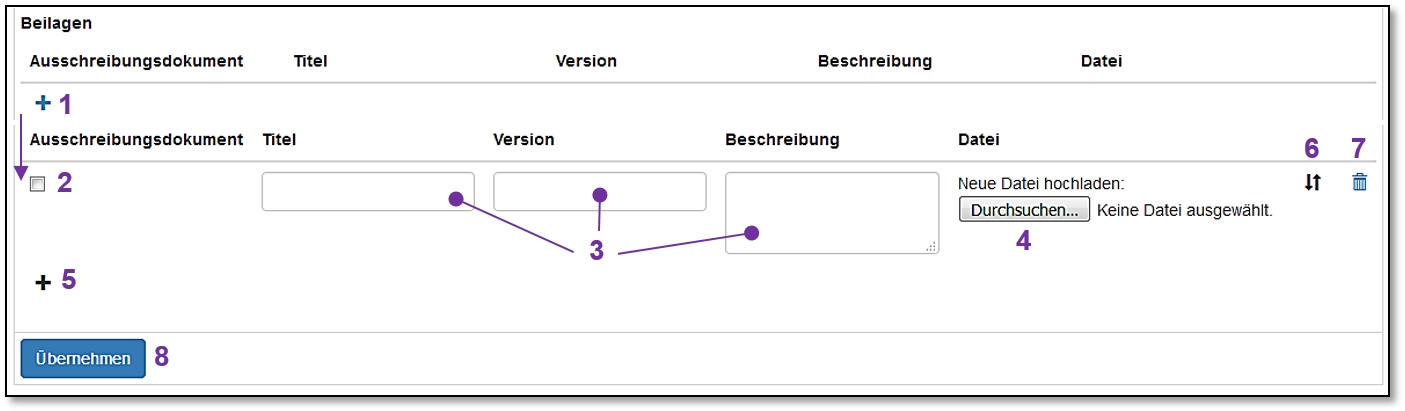
\includegraphics[width=1\linewidth]{../chapters/07_Beschaffungswesen/pictures/7-1-3_OffertanfrageHochladen.jpg}}
\caption{Ajouter une pièce jointe pour l'appel d'offres}
% \label{fig:speciation}
\end{figure}

\begin{itemize}
\item Si la pièce jointe est un document d'appel d'offre (à envoyer avec l'appel d'offres), cochez la case 'Document d'appel d'offre' \col{(2)}
\item Les champs de titre version et description sont des champs de texte libre \col{(3)}. Dans la majorité des cas, il suffit de saisir juste le titre.
\item Cliquez sur 'Parcourir' \col{(4)} pour choisir un fichier à ajouter. Si vous avez sélectionné le mauvais fichier, 
ajouter simplement un nouveau.
\item Cliquez sur le symbole plus \includegraphics[height=12pt]{/Icons/pluszeichen.jpg}-Symbol \col{(5)} pour ajouter des pièces jointes additionnelles.
\item Vous pouvez modifier l'ordre des pièces jointes par glisser-déposer en utilisant les flèches 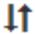
\includegraphics[height=12pt]{/Icons/VertPfeile.jpg} \col{(6)}.
\item Cliquez sur le symbole de poubelle 
\includegraphics[height=12pt]{/Icons/Muelltonne.jpg} \col{(7)} pour supprimer une pièce jointe.
\item Après avoir ajouté les pièces jointes et rempli les données (titre etc.), cliquez sur 'Actualiser' \col{(8)} pour terminer la procédure.
\end{itemize}

\textbf{Remarque :} Le nom du fichier chargé est automatiquement repris dans le champ 'Titre'. Vous pouvez modifier ce champs.

\subsubsection{Étape 4: Envoi de l'appel d'offres}

Dans le masque de modification de l'acquisition se trouve en haut à gauche le symbole d'avion en papier 
\includegraphics[height=12pt]{/Icons/Versandsymbol.jpg}. Cliquez dessus et la page d'envoi s'affiche. A gauche, les soumissionnaires invités sont listés \col{(1)}, au milieu, vous pouvez à nouveau cliquer sur le symbole d'avion en papier 
\includegraphics[height=12pt]{/Icons/Versandsymbol.jpg} \col{(2)} pour générer un e-mail, et à gauche, vous pouvez cliquer sur le symbole de lettre 
\includegraphics[height=12pt]{/Icons/Briefsymbol.jpg} \col{(3)} pour générer un fichier PDF de la lettre que vous pouvez ensuite imprimer.

\begin{figure}[H]
\center{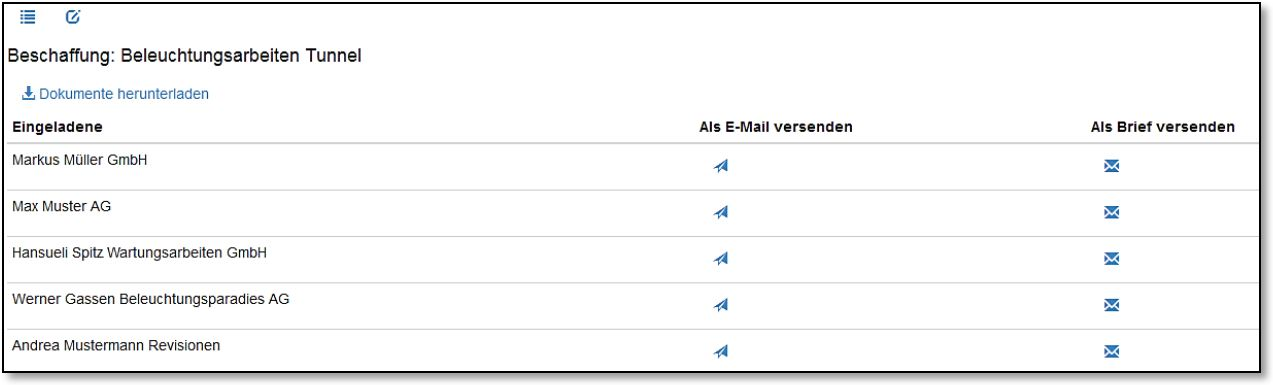
\includegraphics[width=1\linewidth]{714_BeschaffungVersand.jpg}}
\caption{Envoyer l'appel d'offre}
% \label{fig:speciation}
\end{figure}

S'il y a des pièces jointes, cliquez sur 'Télécharger documents' \col{(4)} pour les télécharger. Ceci est uniquement nécessaire si vous avez choisi d'imprimer les documents pour les envoyer avec la lettre d'invitation à l'appel d'offre.

\vspace{\baselineskip}

Quand vous cliquez sur le symbole d'avion en papier 
\includegraphics[height=12pt]{/Icons/Versandsymbol.jpg}, le courriel généré est ouvert dans votre programme de courriels. Contrôlez si les destinataires, le texte, et la signature sont en ordre et complétez le courriel si nécessaire. Les pièces jointes ne seront pas inclues dans l'e-mail, mais un lien pour les télécharger directement depuis la base de données CUBE PA est inclus. De cette manière, des problèmes qui peuvent arriver si les pièces jointes sont trop larges sont évités.

\begin{wrapfigure}[7]{r}{6cm}
\vspace{-15pt}
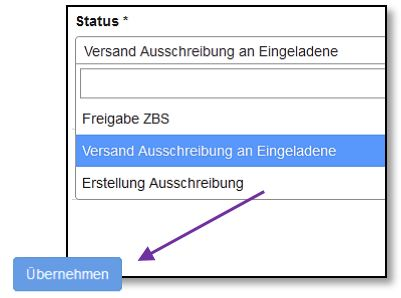
\includegraphics[height=50mm]{714_BeschaffungEingeladene.jpg}
% \caption{Status ändern}
\end{wrapfigure}

Retournez à la liste des acquisitions (menu à gauche, élément 'Fonction d'acquisition', sous-élément 'Acquisitions'), ouvrez l'acquisition en mode de modification en cliquant sur le symbole de crayon 
\includegraphics[height=12pt]{/Icons/Bearbeiten.jpg} et changez l'état de l'acquisition à 'Appel d'offres envoyé'. Cliquez ensuite sur le bouton 'Actualiser'.

\vspace{\baselineskip}

\subsubsection{Étape 5: Réception et chargement des offres}

Dans le menu à gauche, sélectionnez l'élément 'Fonction d'acquisition' puis le sous-élément 'Offres'. La liste des offres s'affiche.

\begin{figure}[H]
\center{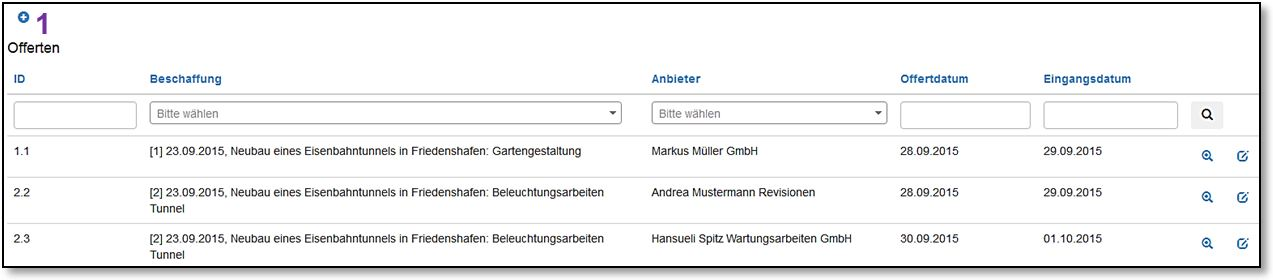
\includegraphics[width=1\linewidth]{715_OfferteUebersicht.jpg}}
\caption{Aperçu des offres}
% \label{fig:speciation}
\end{figure}

Cliquez sur le symbole plus 
\includegraphics[height=12pt]{/Icons/Plussymbol.jpg} \col{(1)} en haut à gauche. Les masque de saisie pour une nouvelle offre s'affiche.

\begin{figure}[H]
\center{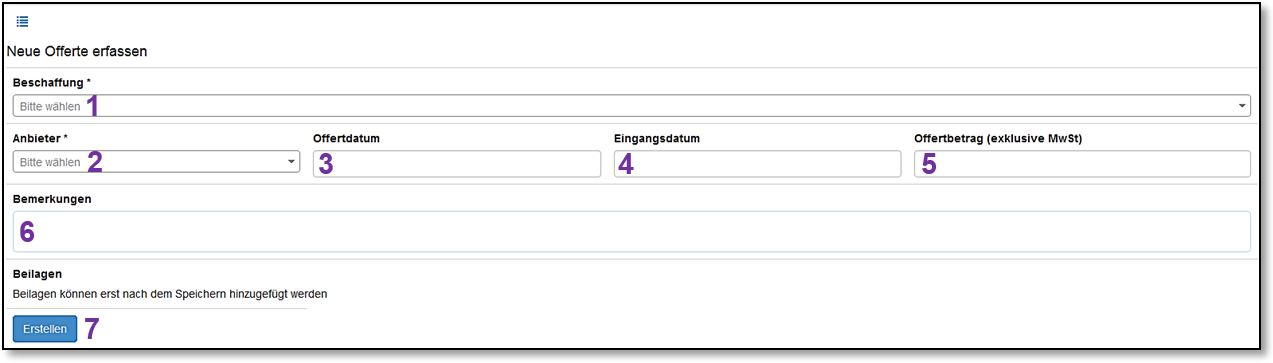
\includegraphics[width=1\linewidth]{715_OfferteErfassen.jpg}}
\caption{Saisir une nouvelle offre}
% \label{fig:speciation}
\end{figure}


Les champs obligatoires sont indiqués par un astérisque *. Saisissez les informations suivants :

\vspace{\baselineskip}

\begin{compactitem}
\item
Acquisition \col{(1)} : Sélectionnez l'appel d'offres (acquisition) auquel l'offre correspond. Seuls les appels d'offres ayant l'état 'Appel d'offres envoyés' apparaissent sur la liste.
\item
Soumissionnaire \col{(2)} : Sélectionnez le soumissionnaire qui a envoyé l'offre. Si l'appel d'offre a été envoyé à un seul soumissionnaire, seul ce dernier figurera sur la liste.
\item
Date de l'offre \col{(3)} : Choisissez la date de l'offre au moyen du calendrier.
\item
Date de réception \col{(4)} : Choisissez la date de réception de l'offre au moyen du calendrier.
\item
Montant \col{(5)} : Indiquez le montant total de l'offre. Seuls des chiffres et un point peuvent être saisis.
\item
Remarques \col{(6)} : Vous pouvez ici saisir du texte libre.
\end{compactitem}

\vspace{\baselineskip}

Cliquez ensuite sur le bouton 'Créer' \col{(7)}. Vous pouvez maintenant charger
l'offre :

\begin{figure}[H]
\center{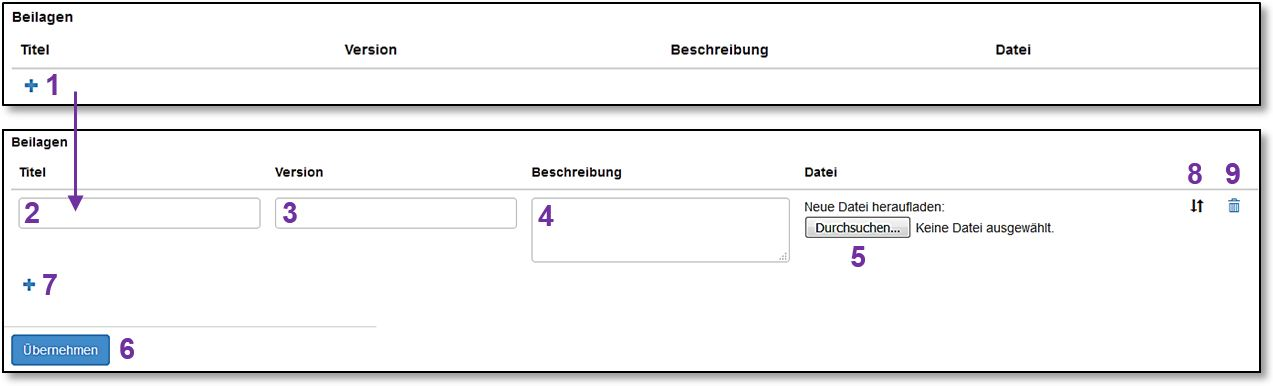
\includegraphics[width=1\linewidth]{715_OfferteHochladen.jpg}}
\caption{Ajouter une offre}
% \label{fig:speciation}
\end{figure}

Cliquez sur le symbole plus 
\includegraphics[height=12pt]{/Icons/Pluszeichen.jpg} \col{(1)} pour ajouter l'offre. Saisissez le titre \col{(2)}, ainsi que la version \col{(3)} et une description \col{(4)} du document en tant que texte libre dans les champs correspondants. Cliquez 'Parcourir' \col{(5)} et sélectionnez le fichier à charger. Si vous avez ajouté le mauvais fichier, ajoutez simplement un nouveau. Cliquez ensuite sur 'Actualiser' \col{(6)} pour enregistrer les données.

\vspace{\baselineskip}

Si l'offre comporte plusieurs documents, cliquez à nouveau sur le symbole plus 
\includegraphics[height=12pt]{/Icons/Pluszeichen.jpg} \col{(7)} et répétez le procédé autant que nécessaire. Vous pouvez modifier l'ordre des documents par glisser-déposer en utilisant le symbole des flèches 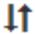
\includegraphics[height=12pt]{/Icons/VertPfeile.jpg} \col{(8)}. Cliquez sur le symbole de poubelle 
\includegraphics[height=12pt]{/Icons/Muelltonne.jpg} \col{(9)} pour supprimer un document.

\vspace{\baselineskip}

\begin{wrapfigure}[7]{r}{6cm}
\vspace{-15pt}
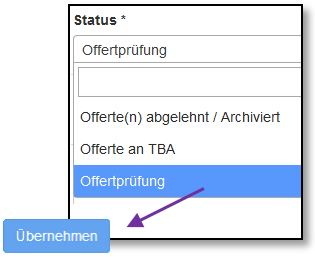
\includegraphics[height=50mm]{715_Offertpruefung.jpg}
% \caption{Status ändern}
\end{wrapfigure}
Retournez à la liste des acquisitions (menu à gauche, élément 'Fonction d'acquisition', sous-élément 'Acquisitions'), ouvrez l'acquisition en mode de modification en cliquant sur le symbole de crayon 
\includegraphics[height=12pt]{/Icons/Bearbeiten.jpg} et changez l'état de l'acquisition à 'Examen des offres'. Cliquez ensuite sur le bouton 'Actualiser'.

\vspace{\baselineskip}

\pagebreak
\subsubsection{Étape 6: Établissement des PVs d'examen des offres et transmission à l'instance de décision}

\begin{wrapfigure}[7]{r}{6cm}
  \vspace{-30pt}      % Grundwert war 20; mit 30 schön oben beim Text ausgerichtet
  \begin{center}
    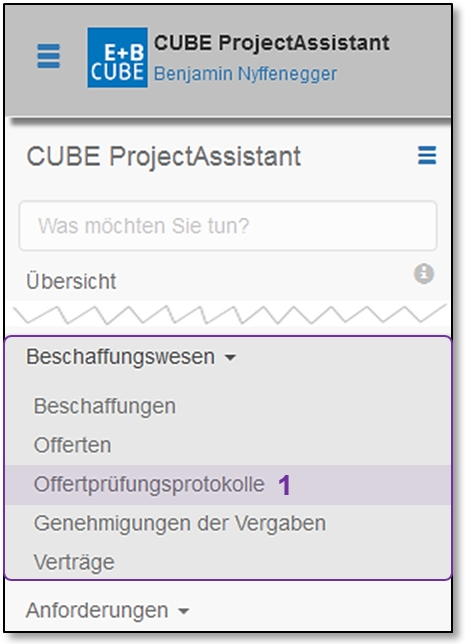
\includegraphics[height=80mm]{../chapters/07_Beschaffungswesen/pictures/7-1-6_Menu_Besch_Offertp.jpg}
  \end{center}
  \vspace{-20pt}
  \caption{Accès aux PVs d'examen des offres}
  \vspace{-10pt}
\end{wrapfigure}

Dans le menu à gauche, sélectionnez l'élément 'Fonction d'acquisition' et le sous-élément 'Procès-verbaux d'examen des offres' \col{(1)}. La liste des PVs d'examen des offres s'affiche.

\begin{center}
\hspace{-15pt}   
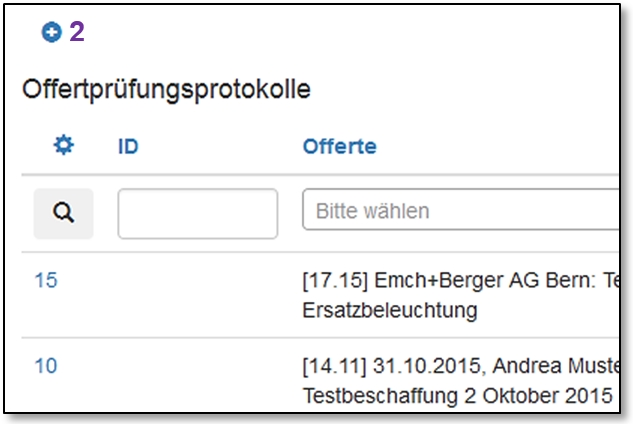
\includegraphics[width=.75\linewidth]{../chapters/07_Beschaffungswesen/pictures/7-1-6_NeuesOffertPruefProtokoll.jpg}
\end{center}

Cliquez sur le symbole plus 
\includegraphics[height=12pt]{/Icons/Plussymbol.jpg} \col{(2)} en haut à gauche. Le masque de saisie d'un nouveau PV d'examen d'offre s'affiche :

\begin{figure}[H]
\center{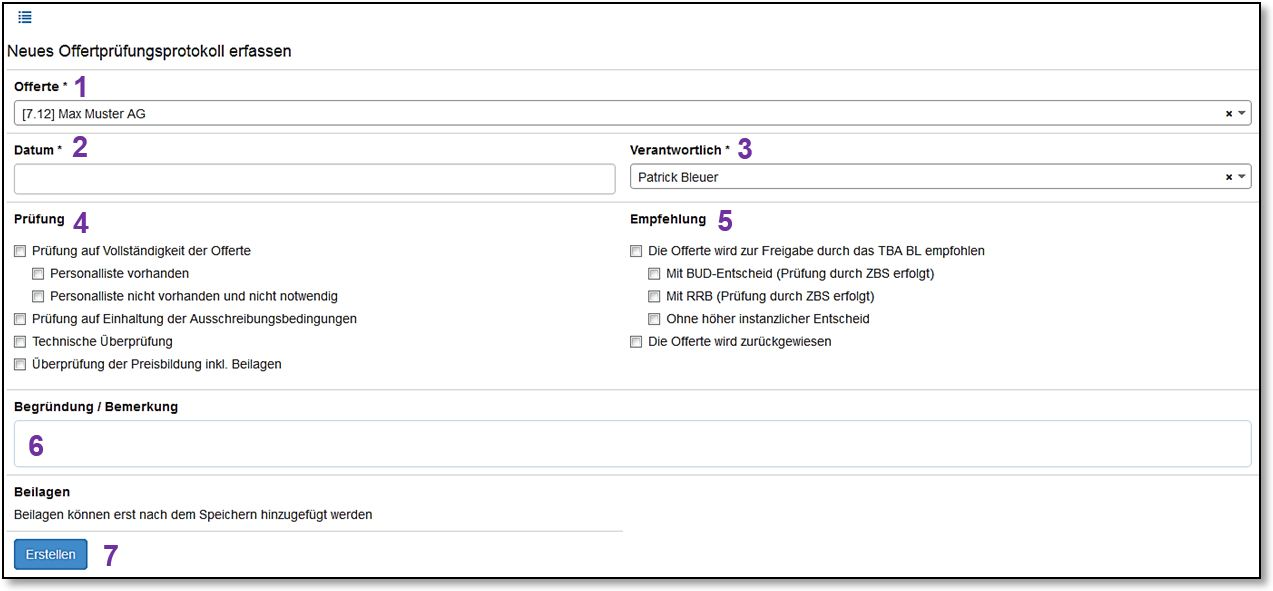
\includegraphics[width=1\linewidth]{716_OffertpruefungsprotokollErfassen.jpg}}
\caption{Saisir un nouveau PV d'examen d'offre}
% \label{fig:speciation}
\end{figure}

Les champs obligatoires sont indiqués par un astérisque *. Saisissez les informations suivants :

\vspace{\baselineskip}

\begin{compactitem}
\item
Dans le premier champ, sélectionnez l'offre à examiner. La liste de sélection \col{(1)} comprend uniquement les offres pour lesquelles un PV d'examen n'existe pas.
\item
\textcolor{black}{Date }\col{(2)} \textcolor{black}{: Saisissez la date d'examen du calendrier. }Par défaut, la date du jour est automatiquement proposée.
\item
Dans le champ 'Responsable' \col{(3)} sélectionnez l'utilisateur responsable du PV. L'utilisateur responsable est celui qui signe le PV d'examen de l'offre.
\item {\sffamily
Sous 'Vérification' \col{(4)} et 'Recommandation' \col{(5)}, cochez les cases qui s'appliquent.}
\item
Si nécessaire, saisissez un texte dans le champ 'Justification / Remarques' \col{(6)}.
\end{compactitem}

\vspace{\baselineskip}

Cliquez sur le bouton 'Créer' \col{(7)}. Vous pouvez maintenant ajouter des pièces jointes.

\begin{figure}[H]
\center{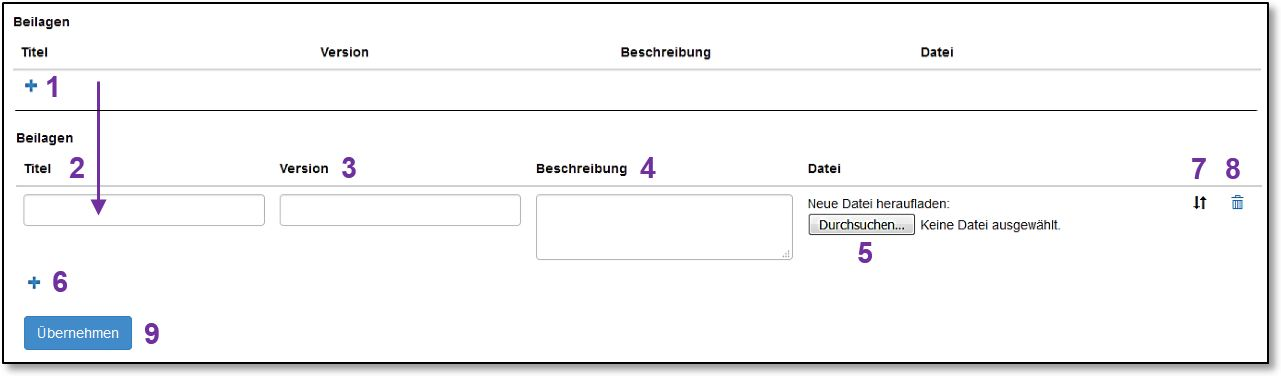
\includegraphics[width=1\linewidth]{716_OffertenpruefungsprotokollBeilagen.jpg}}
\caption{Ajouter des pièces jointes au PV d'examen d'offre}
% \label{fig:speciation}
\end{figure}

Cliquez sur le symbole plus 
\includegraphics[height=12pt]{/Icons/Pluszeichen.jpg} \col{(1)} pour ajouter des pièces jointes. Saisissez le titre \col{(2)}, la version \col{(3)} et une description \col{(4)} en tant que texte libre dans les champs correspondants. Cliquez sur 'Parcourir' \col{(5)} pour charger un fichier. Si vous avez sélectionner le mauvais fichier, sélectionnez simplement un nouveau. Cliquez ensuite sur 'Actualiser' pour enregistrer les donneés. \\
Si vous voulez ajouter des pièces jointes additionnelles, cliquez à nouveau sur le symbole plus 
\includegraphics[height=12pt]{/Icons/Pluszeichen.jpg} \col{(6)} et répétez le procédé autant que nécessaire. Vous pouvez modifier l'ordre des documents par glisser-déposer en utilisant le symbole des flèches 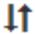
\includegraphics[height=12pt]{/Icons/VertPfeile.jpg} \col{(7)}. Cliquez sur le symbole de poubelle 
\includegraphics[height=12pt]{/Icons/Muelltonne.jpg} \col{(8)} pour supprimer un document.

\vspace{\baselineskip}

\begin{wrapfigure}[7]{r}{5cm}
\vspace{-15pt}
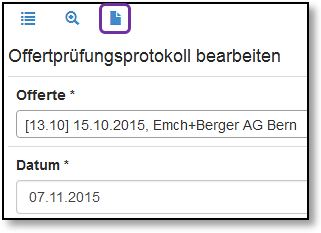
\includegraphics[height=40mm]{716_OffertpruefungsprotokollPDFgen.jpg}
% \caption{Status ändern}
\end{wrapfigure}
Cliquez sur 'Actualiser' \col{(9)} pour enregistrer les données. Cliquez en haut à gauche sur 
le symbole de feuille \includegraphics[height=12pt]{/Icons/BLattsymbol.jpg} pour générer le procès-verbal d'offre en tant que fichier PDF. Imprimez le document et faites le signer. Scannez ensuite le document signé et ajoutez-le comme pièce jointe au procès-verbal 
d'examen d'offre. Le procès-verbal original est ensuite à envoyer à l'instance de décision avec l'offre originale.

\vspace{\baselineskip}

\begin{wrapfigure}[7]{r}{6cm}
\vspace{-15pt}
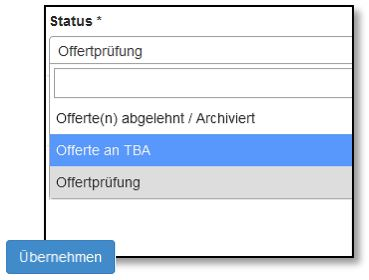
\includegraphics[height=50mm]{716_BeschaffungStatus.jpg}
% \caption{Status ändern}
\end{wrapfigure}
Retournez à la liste des acquisitions (menu à gauche, élément 'Fonction d'acquisition', sous-élément 'Acquisitions'), ouvrez l'acquisition en mode de modification en cliquant sur le symbole de crayon 
\includegraphics[height=12pt]{/Icons/Bearbeiten.jpg} et changez l'état de l'acquisition à 'Offre chez X'. Cliquez ensuite sur le bouton 'Actualiser'.

\vspace{\baselineskip}

La procédure est suspendue dans CUBE PA jusqu'à ce que l'instance de décision aura conclu le contrat et l'aura fait signé par les deux parties. Le contrat doit ensuite être saisi dans CUBE PA pour rendre son contenu accessible.

\subsubsection{Étape 7: Approbation de la procédure par une position d'ordre supérieur}

Si, dans le PV d'examen d'offre, vous avez cocher la case nécessitant que la décision soit approuvée par une position d'ordre supérieure (par exemple un conseil gouvernemental), fixez l'état de l'acquisition à 'Décision position d'ordre supérieur'.

\subsubsection{Étape 8: Établissement d'un contrat}

\begin{wrapfigure}[7]{r}{6cm}
  \vspace{-30pt}      % Grundwert war 20; mit 30 schön oben beim Text ausgerichtet
  \begin{center}
    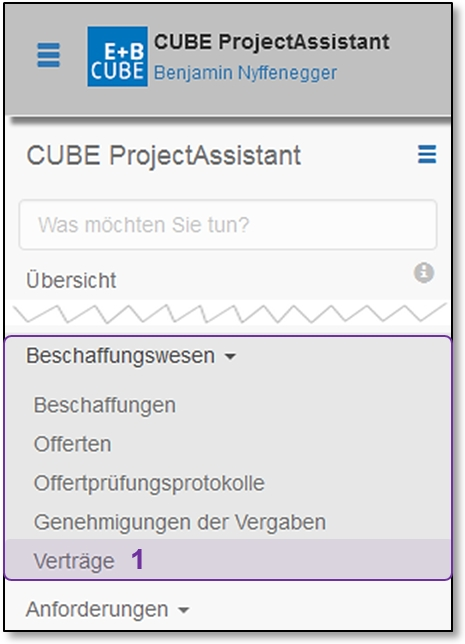
\includegraphics[height=80mm]{../chapters/07_Beschaffungswesen/pictures/7-1-8_Menu_Besch_Vertraege.jpg}
  \end{center}
  \vspace{-20pt}
  \caption{Accès à la liste des contrats}
  \vspace{-10pt}
\end{wrapfigure}

Les contrats sont enregistrés dans TDCost (comme base pour le contrôle des coûts) aussi bien que dans CUBE PA, afin de pleinement documenter l'avancement de l'acquisition et de pouvoir rendre le contenu des contrats accessible. Si possible, saisissez le contrat d'abord dans TDCost, afin d'avoir à disposition toutes les informations 
nécessaires de CUBE PA.

\begin{center}
\hspace{-55mm}   
\includegraphics[width=.4\linewidth]{../chapters/07_Beschaffungswesen/pictures/7-1-8_NeuerVertrag.jpg}
\end{center}

\vspace{\baselineskip}

Dans le menu à gauche, sélectionnez l'élément 'Fonction d'acquisition' et le sous-élément 'Contrats' \col{(1)}. La liste des contrats s'affiche.

\vspace{\baselineskip}

Cliquez sur le symbole plus \includegraphics[height=12pt]{/Icons/Plussymbol.jpg} \col{(2)} en haut à gauche. Le masque de saisie pour un nouveau contrat s'affiche. Le symbole de liste \includegraphics[height=12pt]{/Icons/Listensymbol_zurueck.jpg} \col{(3)} vous permet de retourner à la liste / l'aperçu.

\begin{figure}[H]
\center{\includegraphics[width=1\linewidth]{718_VertragErfassen.jpg}}
\caption{Ajouter un nouveau contrat}
% \label{fig:speciation}
\end{figure}

Les champs obligatoires sont indiqués par un astérisque *. Saisissez les informations suivants :

\vspace{\baselineskip}

\begin{compactitem}
\item {\sffamily\color{black}
Sous 'Offre', choisissez l'offre qui sert de base pour ce contrat. Seuls les offres des acquisitions en cours figurent sur la liste de sélection.}
\item
Le champ 'Titre du contrat' est automatiquement rempli à partir des informations de l'offre. Vous pouvez néanmoins le modifier.
\item
Le champ 'Projet / Sous-projet' est automatiquement rempli à partir des informations de l'acquisition. Vous pouvez néanmoins modifier ou compléter la sélection.
\item
La 'Date du contrat' peut être choisie à partir d'un calendrier.
\item
Les champs 'Date de début' et 'Date de fin' peuvent également être remplis à partir d'un calendrier. Il s'agit des dates de début et de fin des prestations.
\item
Le 'Client' est à choisir à partir d'une liste, et le 'Mandataire' est automatiquement fixé sur la base des données de l'offre.
\item
Le 'Montant du contrat' est également automatiquement repris des données de l'offre. Vous pouvez néanmoins le modifier, par exemple si seule une partie des prestations offertes fait partie du contrat.
\item
Les champs 'Numéro de référence externe (Contrat)' et 'Etat externe (Contrat) font référence à la classification du contrat par d'autres systèmes (par exemple TDCost). Si le contrat n'est pas enregistré dans un autre système, fixez l'état à 'indéfini'.
\item
Sous 'Contrôleur', sélectionnez l'utilisateur responsable du suivi du contrat, et choisissez également un 'Contrôleur remplaçant'.
\item
Dans le champ 'Contenu / Prestation', les données de l'offre sont automatiquement reprises. Vous pouvez néanmoins les modifier, par exemple si seule une partie des prestations offertes fait partie du contrat.
\item
Le champ 'Remarques' est un champ de texte libre.
\end{compactitem}

\vspace{\baselineskip}

Cliquez sur le bouton 'Créer' \col{(4)} et vous pouvez ensuite charger le contrat.

\begin{figure}[H]
\center{\includegraphics[width=1\linewidth]{718_VertragHochladen.jpg}}
\caption{Ajouter un contrat}
% \label{fig:speciation}
\end{figure}

Cliquez sur le symbole plus \includegraphics[height=12pt]{/Icons/Pluszeichen.jpg} \col{(1)} pour ajouter le contrat. Saisissez le titre \col{(2)}, la version \col{(3)} et une description du document \col{(4)} en tant que texte libre dans les champs correspondants. Cliquez 'Parcourir' \col{(5)} et sélectionnez le fichier pour le charger. Si vous avez sélectionné le mauvais fichier, choisissez simplement un nouveau. Cliquez ensuite sur 'Actualiser' \col{(6)} pour enregistrer les données.

\vspace{\baselineskip}

Si le contrat comporte plusieurs documents, cliquez à nouveau sur le symbole plus \includegraphics[height=12pt]{/Icons/Pluszeichen.jpg} \col{(7)} et répétez le procédé autant que nécessaire. Vous pouvez modifier l'ordre des documents par glisser-déposer en utilisant le symbole des flèches \includegraphics[height=12pt]{/Icons/VertPfeile.jpg} \col{(8)}. Cliquez sur le symbole de poubelle \includegraphics[height=12pt]{/Icons/Muelltonne.jpg} \col{(9)} pour supprimer un document.
\vspace{\baselineskip}

Retournez à la liste des acquisitions (menu à gauche, élément 'Fonction d'acquisition', sous-élément 'Acquisitions'), ouvrez l'acquisition en mode de modification en cliquant sur le symbole de crayon \includegraphics[height=12pt]{/Icons/Bearbeiten.jpg} et changez l'état de l'acquisition à 'Acquisition terminée'. Cliquez ensuite sur le bouton 'Actualiser'.

\vspace{\baselineskip}

\textbf{Ajouter un contrat additionnel à une offre existante.}

Si vous avez besoin d'ajouter un contrat additionnel à une offre pour laquelle il existe déjà un contrat, par exemple parce qu'une autre prestation partielle est à fournir, vérifiez d'abord l'état de l'acquisition dans la liste des acquisitions. Si ce dernier est 'Acquisition terminée', changez le à 'Signature X / Envoi' pour que l'offre puisse être sélectionnée quand le contrat est ajoutée. Une  fois le nouveau contrat ajouté, refixez l'état à 'Acquisition terminée'.

\subsubsection{Traiter une offre pour laquelle il n'y a pas eu d'appel d'offres}

Il se peut que vous deviez ajouter une offre pour laquelle il n'y a pas eu d'appel d'offres qui a été envoyé. Ceci peut être le cas si par exemple il est agréé à une séance qu'une personne doit envoyer une offre, ou qu'une personne doit envoyer un avenant à un contrat existant. Dans ces cas, procédez comme suit :


\begin{itemize}
\item
Initialisez une acquisition comme décrit à l'étape 2, sans saisir les informations liées à l'envoi de l'appel d'offres. Si l'offre est un supplément, choisissez l'offre de base dans le champ 'Supplément pour acquisition'.
\item
Sautez les étapes 3 et 4.
\item
Saisissez l'offre comme indiqué à l'étape 5. Cette étape et les suivantes se déroulent exactement de la même manière que si l'offre a été faite suite à un appel d'offres.
\end{itemize}

\subsection{Flux de travail pour des procédures sur invitation ou des procédures ouvertes}

Un flux de travail type pour des acquisitions en procédures sur invitation ou en procédures ouvertes suivra plus tard.

